\section{Классическая модель Барро-Гордона}
\label{sec:domain}

\paragraph{} Классическая модель Барро-Гордона рассматривает правительство (в лице некоторого одного политика), которое принимает решение о мерах воздействия на экономику основываясь на двух факторах. Первый фактор являет собой суммарную функцию благосостояния вида

\begin{equation}
 \label{eq:sec:domain:main}
W=\sum_{t=0}^{\infty}\beta^t w_t = \sum_{t=0}^{\infty}\beta^t\left(y_t-\frac{\lambda\pi^2}{2}\right), \quad 0<\beta<1,
\end{equation}
где $\beta^t$ - значимость $t$-ого периода для благосотояния политика, $w_t$ - функция благосостояния политика в $t$-ом периоде. При этом взаимосвязь между инфляцией и безработицей задается кривой Лукаса
\begin{equation}
	\label{eq:sec:domain:main1}
	y=y^*+\alpha(\pi-\pi^\beta).
\end{equation}\\
Второй фактор принятия решения -- это оценка общественностью действий правительства в виде поддержки или недоверия. Такая оценка в модели задается через инфляционные ожидания, которые формируются в период $t$ следующим образом:
\begin{equation}
\label{eq:sec:domain:main2}
\pi_t = \left\{  \begin{array}{l l}
{\pi}, & \forall t:\pi_t=\tilde{\pi_t}, \\ 
\frac{\alpha}{\lambda}, & \exists s < t : \pi_s \ne \tilde{\pi_s},
\end{array} \right. 
\end{equation}
где $\tilde{\pi}$ - уровень инфляции, который политик обещают достичь в результате воздействия на экономику.
\\

Как следует из~(\ref{eq:sec:domain:main2}), если политик ведет себя честно, то общественность ему доверяет и ожидает обещанный им уровень инфляции. Если политик хотя бы раз, обманув ожидания, провел не ту политику, которую обещал, то общественность ему не верит. В таком случае она ожидает отличный от обещанного уровень инфляции, который составляет $\frac{\alpha}{\lambda}$ , поскольку полагает, что в случае обмана политик будет стремиться к тому, чтобы в экономике установился именно этот уровень инфляции.
\\

Действительно, в случае обмана политик выберет такой уровень инфляции, который будет максимизировать его функцию благосостояния в этом периоде (допустим, в периоде $s$). Поскольку, согласно \eqref{eq:sec:domain:main}-\eqref{eq:sec:domain:main2}, функция благосостояния периода $s$ при $\pi_s\ne\tilde{\pi}$ имеет вид

\begin{equation}
	\label{eq:sec:domain:main3}
	w_s=y^*\alpha\left(\pi_s - \frac{\lambda\pi^2_s}{2} \right),
\end{equation}

то максимизирующий её уровень инфляции будет равен величине $\frac{\alpha}{\lambda}$, что следует из первого условия максимизации.\\

Так как репутация политика влияет на инфляционные ожидания общественности, то, согласно  \eqref{eq:sec:domain:main}-\eqref{eq:sec:domain:main1}, репутация влияет также и на его общую функцию благосостояния. Предположим, что политик ведет себя честно, то есть проводит ту политику, которую обещал. Тогда его общая функция благосостояния принимает вид

\begin{equation}
	w^{fair} = \frac{1}{(1-\beta)} \left( y^*-\frac{\lambda\pi^2}{2} \right),
\end{equation}

поскольку в этом случае, согласно \eqref{eq:sec:domain:main}-\eqref{eq:sec:domain:main2},  функция благосостояния для любого периода $t$ имеет вид

\begin{equation}
w^{fair}_t = y^*-\frac{\lambda\pi^2}{2}.
\end{equation}

Если политик решит обмануть ожидания общественности в какой-то (допустим в нулевой) период времени, то в этом случае, согласно \eqref{eq:sec:domain:main}-\eqref{eq:sec:domain:main2}, его функция благосостояния в нулевой период составит

\begin{equation}
w^{deception}_0 = y^*-\frac{\alpha^2}{2\lambda}-\alpha\tilde{\pi},
\end{equation}

а во все последующие периоды вследствие недоверия населения общественности
\begin{equation}
w^{deception}_0 = y^*-\frac{\alpha^2}{2\lambda}.
\end{equation}

Следовательно, общая функция благосостояния политика в случае нарушения данных обещаний имеет вид

\begin{equation}
W^{deception} = \frac{1}{(1-\beta)}y^*+\frac{(1-2\beta)\alpha^2}{(1-\beta)2\lambda}-\alpha\tilde{\pi},
\end{equation}

Очевидно, что политику имеет смысл вести себя честно только при условии $W^{fair} > W^{deception}$ , в противном случае он выигрывает больше от невыполнения данных ранее обещаний.
\\

Выведем условия, при которых политик ведет себя честно, не обманывая ожидания населения. Воспользуемся для этого графической интерпретацией этой проблемы: построим графики выигрыша и проигрыша политика в случае обмана и найдем области, в которых выигрыш будет больше проигрыша и наоборот.

\begin{figure}[h]
	
	\begin{subfigure}{0.5\textwidth}
		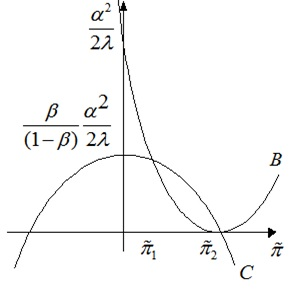
\includegraphics[width=0.9\linewidth]{pic1.jpg} 
		\caption{}
		\label{fig:pic1}
	\end{subfigure}
	\begin{subfigure}{0.5\textwidth}
		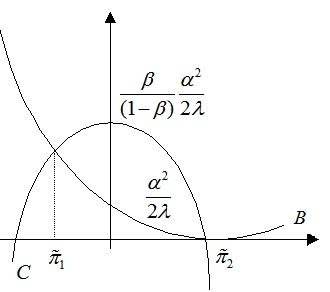
\includegraphics[width=0.9\linewidth]{pic2.jpg}
		\caption{}
		\label{fig:pic2}
	\end{subfigure}
	
	\caption{}
	\label{fig:image2}
\end{figure}

Если политик обманывает ожидание общественности в нулевой момент времени, то выигрыш он получает за счет того, что в нулевой момент времени обманул ожидания общественности, а проигрыш – что в дальнейшем общественность перестает ему доверять и всегда ожидает больший уровень инфляции, было объявлявленно.
\\

Следовательно, выигрыш обманывающего население в нулевой момент времени политика

\begin{equation}
B=w^{deception}_0 - w^{fair}_0 = \frac{\lambda\pi^2}{2}+\frac{\alpha^2}{2\lambda}-\alpha\tilde{\pi}
\end{equation}

является квадратичной функцией от объявляемого уровня инфляции. Эта функция достигает минимума $B=0$  в точке $\tilde{\pi}=\frac{\alpha}{\lambda}$. При $\tilde{\pi}=0$  выигрыш равен $\frac{\alpha^2}{\lambda}$.
\\

Проигрыш обманывающего население в нулевой момент времени политика также является квадратичной функцией от объявляемого уровня инфляции, поскольку

\begin{equation}
	\label{eq:sec:domain:main4}
C=\sum_{t=1}^{\infty} \beta^t(w^{deception}_t - w^{fair}_t) = -\frac{\lambda\tilde{\pi}^2}{2}+\frac{\alpha^2}{2\lambda}.
\end{equation}



Функция, задаваемая выражением \eqref{eq:sec:domain:main4}, описывает параболу, достигающую максимума $C=\frac{\beta}{(1-\beta)}\frac{\alpha^2}{2\lambda} $  в точке   $\tilde{\pi}=0$. Значение функции $С$ равняется нулю, когда уровень инфляции составляет $\tilde{\pi}\pm\frac{\alpha}{\lambda}$.
\\



Взаиморасположение графиков потерь и выигрыша обманывающего общественность в нулевой момент времени политика зависит от того, больше или меньше единицы величина $\frac{\beta}{1-\beta}$.

Если   $\frac{\beta}{1-\beta}<1$, то есть  $\beta<\frac{1}{2}$, то функция потерь и функция выигрыша пересекаются в точках  $\tilde{\pi}_1>0$ и $\tilde{\pi}_2>0$ \eqref{fig:pic1}, причем  $\tilde{\pi}_1~=~\frac{\alpha(1-2\beta)}{\lambda}$? $\tilde{\pi}_2~=~\frac{\alpha}{\lambda}$. \\
Если  $\frac{\beta}{1-\beta}>1,$  то есть  $\beta>\frac{1}{2},$  то функция потерь и функция выигрыша пересекаются в точках   $\tilde{\pi}_1<0$, $\tilde{\pi}_2>0$ ~(\ref{fig:pic2}).
//

Таким образом, из проведенного анализа следует, что поведение политика (будет он выполнять обещания или нет) зависит от его отношения к репутации. Если для него репутация не важна, будущее мало влияет на его функцию благосостояния $\beta<\frac{1}{2}$, то политику не выгодно вести себя честно. Поскольку, как видно из \eqref{fig:pic1}, существует достаточно невысокий уровень инфляции $\tilde{\pi}\in\left(0;\frac{\alpha(1-2\beta)}{\lambda} \right)$ , обещая который он может выиграть больше в результате обмана (по сравнению с честным поведением). Если для политика его репутация важна, будущее значимо для его благосостояния $\beta<\frac{1}{2}$ , то ему имеет смысл вести себя честно. Поскольку, как видно из \eqref{fig:pic2}, не существует уровня инфляции близкого к нулю, обещая который он может получить большую реализацию своих целей в результате обмана по сравнению с честным поведением.